\section{Implementation}
\label{sec:implementation}

In this assignment, we implemented two types of recurrent neural networks from scratch using PyTorch: a vanilla RNN and a GRU (Gated Recurrent Unit). The purpose was to compare their internal structures and performance on a sequence classification task. Our implementations focused on constructing the forward and backward passes manually within custom PyTorch modules.

\textbf{Vanilla RNN.} The vanilla RNN was implemented in \texttt{RNN\_skeleton.py}. We completed the \texttt{forward()} and \texttt{backward()} methods under the \texttt{RNNCell} class. In the forward pass, we iteratively updated the hidden state $h_t$ using the equation $h_t = \tanh(W_{ih}x_t + W_{hh}h_{t-1} + b)$. In the backward pass, we backpropagated the gradients through time, applying the chain rule to compute gradients with respect to weights and inputs.

\textbf{GRU.} The GRU was implemented in \texttt{GRU\_skeleton.py}. We filled in the \texttt{forward()} and \texttt{backward()} functions for the \texttt{GRUCell} class. The forward computation followed the equations:
\begin{align*}
  z_t &= \sigma(W_{xz}x_t + W_{hz}h_{t-1} + b_z) \\
  r_t &= \sigma(W_{xr}x_t + W_{hr}h_{t-1} + b_r) \\
  \tilde{h}_t &= \tanh(W_{xh}x_t + W_{hh}(r_t \odot h_{t-1}) + b_h) \\
  h_t &= (1 - z_t) \odot h_{t-1} + z_t \odot \tilde{h}_t
\end{align*}
In the backward pass, we derived the gradients of each gate by applying the chain rule over time, taking special care with the Hadamard product and nonlinearities.

\textbf{Training and Evaluation.} We trained both models using cross-entropy loss and the Adam optimizer. Each model was trained for 10 epochs. Final performance was evaluated using test accuracy. We also visualized the accuracy progression during training.

\begin{figure}[h]
\centering
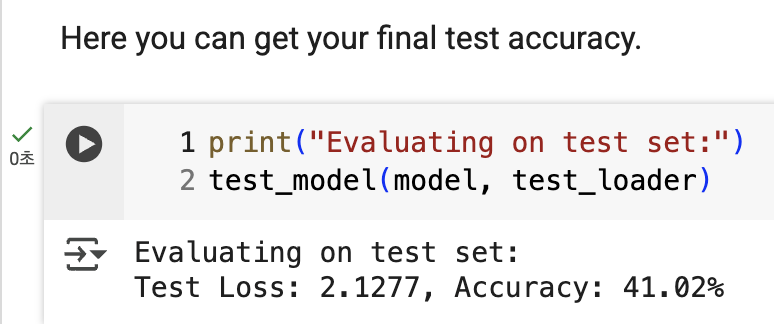
\includegraphics[width=0.8\linewidth]{Vanilla_RNN_accuracy.png}
\caption{Test accuracy of the Vanilla RNN. Final accuracy: 41.02\%.}
\end{figure}

\begin{figure}[h]
\centering
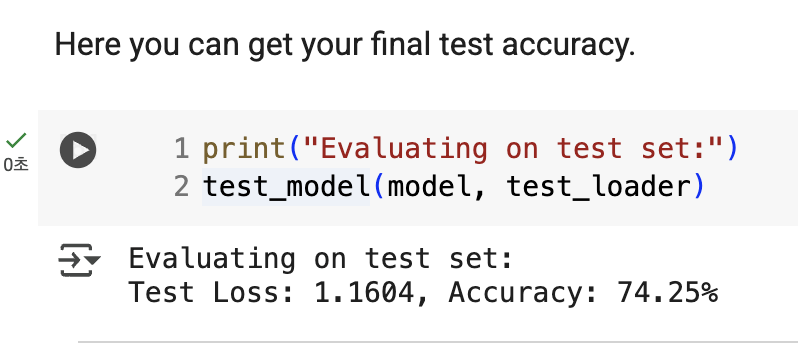
\includegraphics[width=0.8\linewidth]{GRU_accuracy.png}
\caption{Test accuracy of the GRU. Final accuracy: 74.25\%.}
\end{figure}

\section{Discussion}
\label{sec:discussion}

Our experimental results highlight the significant performance gap between vanilla RNNs and GRUs in sequence classification tasks. The vanilla RNN achieved a test accuracy of only 41.02\%, whereas the GRU reached 74.25\%. This large gap demonstrates the impact of gating mechanisms in improving the learning capability of recurrent models.

We observed that the GRU was more stable during training and less sensitive to vanishing gradients, likely due to its reset and update gates. These gates allowed the model to retain and forget information dynamically, helping it capture long-term dependencies better than the vanilla RNN.

Additionally, both models were trained under the same hyperparameter settings to ensure a fair comparison. The GRU consistently converged faster and to a better local minimum. These findings support the argument that architectural improvements like gating mechanisms are crucial for deep sequential learning.

In future work, it would be beneficial to explore LSTM models or apply attention mechanisms to further enhance performance in text classification tasks.

